\clearpage
\subsubsection{逻辑化简法}
\label{subsubsec:lab4-task1-logic-minimization}

\paragraph{非法点函数的构造与化简}

逐点排除法中，每个非法点都需要一条不等式。逻辑化简法进一步考虑将多个非法点合并处理：先构造一个八输入布尔函数，使其在非法点上取1，在合法点上取0，再使用Espresso将这个函数化简为若干乘积项。每个乘积项对应一个逻辑立方体，其中部分坐标固定为0或1，其余坐标可以任意取值。

本实验在\texttt{logic\_minimization.py}中通过PyEDA提供的\texttt{espresso\_exprs}接口调用Espresso。\footnote{PyEDA的Espresso接口及两层逻辑化简说明：\url{https://pyeda.readthedocs.io/en/latest/2llm.html}。}程序按公共位序建立8个布尔变量，对每个零值位置生成一个最小项，再将所有最小项取或：
\par\noindent\begin{minipage}{\linewidth}
\begin{lstlisting}
variables = exprvars("x", 8)
minterms = []
for a in range(SIZE):
    for b in range(SIZE):
        if table[a][b] == 0:
            point = bits(a, b)
            minterms.append(And(*(
                variable if value else ~variable
                for variable, value in zip(variables, point)
            )))

forbidden_function = Or(*minterms).to_dnf()
minimized, = espresso_exprs(forbidden_function)
\end{lstlisting}
\end{minipage}\par

化简后的析取范式仍表示同一组非法点。程序从\texttt{minimized.to\_dnf().cover}中逐项读取文字：正文字表示该位固定为1，负文字表示该位固定为0，没有出现的变量用\texttt{None}表示通配位。这里根据文字的唯一标识找到原来的变量下标，使化简前后的坐标始终对应$(a_3,a_2,a_1,a_0,b_3,b_2,b_1,b_0)$。

\paragraph{立方体到线性约束的转换}

对于一个非法立方体，只要当前点有一个固定坐标与它不同，该点就位于立方体之外。因此，对固定为0的位置累加$z_j$，对固定为1的位置累加$1-z_j$，并要求总和至少为1。通配位不参与求和。关键代码为：
\begin{lstlisting}
z = model.addVars(8, vtype=gp.GRB.BINARY, name="z")
for cube in cubes:
    model.addConstr(gp.quicksum(
        z[j] if value == 0 else 1 - z[j]
        for j, value in enumerate(cube) if value is not None
    ) >= 1)
\end{lstlisting}

这样，一条不等式可以排除一个立方体覆盖的多个非法点。Espresso负责构造较紧凑的非法点覆盖，Gurobi负责求解转换后的线性约束，两者在程序中依次执行。模型仍只有8个原始二进制变量。

\clearpage
\paragraph{实验结果与分析}

代码运行结果如图~\ref{fig:lab4-task1-logic-minimization}所示。
\begin{figure}[H]
    \centering
    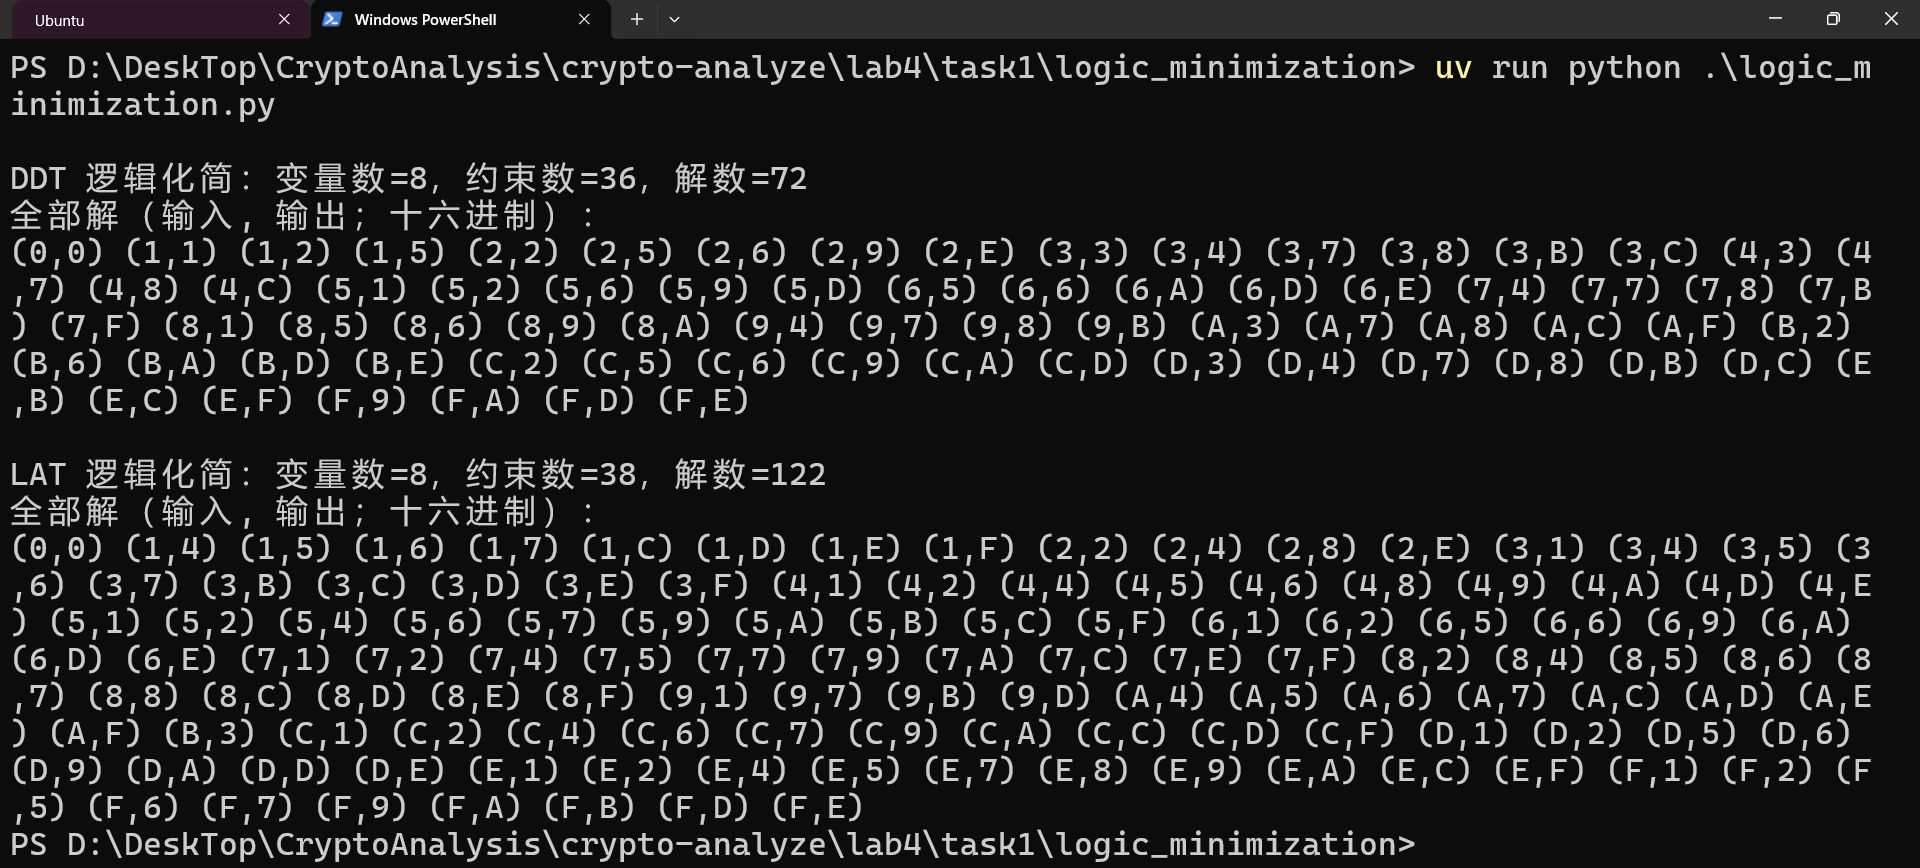
\includegraphics[width=\textwidth]{figures/task1/logistic_minimization.png}
    \caption{Espresso逻辑化简后由Gurobi枚举得到的结果}
    \label{fig:lab4-task1-logic-minimization}
\end{figure}

本次Espresso调用为DDT非法点集生成36个立方体，为LAT非法点集生成38个立方体，因此两个模型分别包含36条和38条不等式。相比逐点排除法的184条和134条，逻辑化简在保留8个变量的同时减少了约束数量。

Gurobi分别枚举出72个差分合法点和122个线性合法点，具体输入输出对与前两种方法一致，也与DDT、LAT中的非零位置一致。这说明立方体合并及其线性约束转换保持了原有的二进制解集。本实验使用的是PyEDA中的Espresso化简接口，36和38记录本次得到的覆盖规模，不能据此认定约束数量已经达到全局最少。
